\section{Relative Depth of the Optimal Layer}
\label{sec:ch8-depth}

\phantomsection\label{rq:ch8-rq3-intro}
\begin{rqbox}[RQ3]
Does the optimal probe layer fall at a consistent relative depth across different LLMs?
\end{rqbox}


\noindent To answer \hyperref[rq:ch8-rq3-intro]{\textbf{RQ3}}, this section measures where the optimal layer of each run falls in the stack of layers of its model (Section~\ref{subsec:block}), expressed as a fraction of the number of layers, called the \emph{relative depth}. Section~\ref{sec:ch7-results} reports the optimal layer of each run, the layer at which the probe reaches its highest accuracy. That layer index does not compare directly across models, because the layer count in the pool ranges from 30 to 80, so a specific layer does not mark the same depth in every model. A relative depth that is similar across the models indicates that the routing signal concentrates at the same relative depth in every model.

\subsection{Relative Depth of the Optimal Layer per Run}
\label{subsec:ch8-depth-values}

Each optimal layer is divided by the last layer index, which places it in $[0, 1]$ and gives its relative depth. This rescaling makes the positions comparable across models. Figure~\ref{fig:ch8-depth} plots the relative depth of the optimal layer for the fourteen runs.

\begin{figure}[htbp]
    \centering
    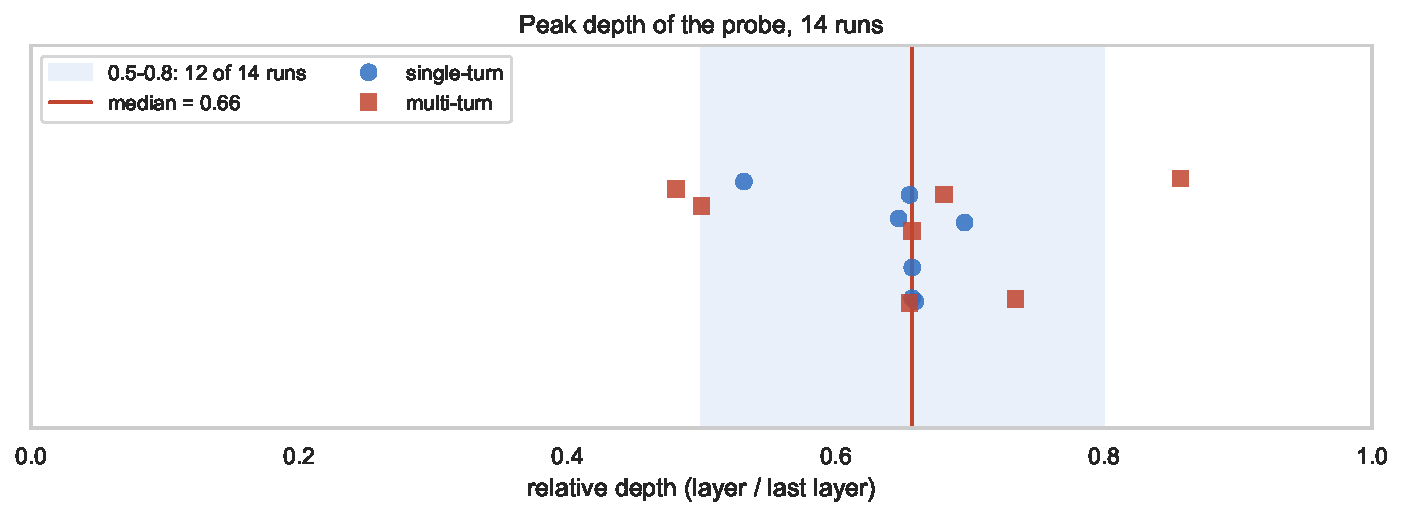
\includegraphics[width=\textwidth]{images/plots/overview/overview_depth.pdf}
    \caption[Relative depth of the probe's optimal layer]{Relative depth of the probe's optimal layer, fourteen runs.}
    \label{fig:ch8-depth}
\end{figure}

The median relative depth is 0.66, with quartiles at 0.65 and 0.68. Twelve of the fourteen runs fall between 0.5 and 0.8. The two remaining runs fall outside that range: Llama 3.3 70B multi-turn at 0.48, 0.02 below the lower bound, and Qwen3 8B multi-turn at 0.86, 0.06 above the upper bound. The single-turn and the multi-turn runs give the same median, so the number of turns does not move the relative depth of the optimal layer, but the two groups differ in spread: the standard deviation of the relative depth is 0.05 for the single-turn runs and 0.13 for the multi-turn runs. Section~\ref{subsec:ch8-multi-turn} relates the larger multi-turn drop in probe accuracy to a less separable representation of the sub-agents in the multi-turn hidden states, and the same reduced separability could also explain why the multi-turn relative depth is less consistent across models.

Ratnakar et al. note that deeper layers dominate in typical probing results, but their own LatentGate results differ: the optimal layer falls at a relative depth of 0.25 to 0.50 \cite{ratnakarLatentGateLowLatencySemantic2026}. They give as a likely reason that their agent-routing task requires broad topic discrimination rather than fine-grained linguistic analysis. The median relative depth of 0.66 here is larger, so the optimal layer falls in the second half of the layer stack. The routing task in this work requires deciding which of several constraints binds on a shared scenario, a finer-grained judgment than topic-level agent selection. Following the explanation of Ratnakar et al., this finer-grained judgment may be the reason why the optimal layer falls deeper than in LatentGate.

\subsection{Answer to RQ3}
\label{subsec:ch8-rq3-answer}

\phantomsection\label{rq:ch8-rq3}
\begin{rqbox}[RQ3]
Does the optimal probe layer fall at a consistent relative depth across different LLMs?
\end{rqbox}


\noindent Yes. The relative depth of the optimal layer lies between 0.5 and 0.8 in twelve of the fourteen runs, with a median of 0.66 that is the same on the single-turn and on the multi-turn dataset.

The consistency is lower in the multi-turn setting. Both runs outside the 0.5 to 0.8 band are multi-turn, Llama 3.3 70B at 0.48 and Qwen3 8B at 0.86, and the standard deviation of the relative depth is 0.13 on the multi-turn dataset against 0.05 on the single-turn dataset.

The claim that the optimal layer occurs at a consistent relative depth is limited to the pool of models analyzed in this work, which is too small to provide a valid generalization.

\FloatBarrier
